Elektrisches Rauschen stammt im Wesentlichen daher, dass elektrische Ladung nicht kontinuierlich verteilt ist und daher statistische Effekte der Ladungsträger zu Rauschen führen.
Rauschen wird in der Regel als Varianz einer Strom- oder Spannungsquelle normiert auf das Frequenzband angegeben, die Einheit ist dann $\SI{}{\ampere^2\per\sqrt\hertz}$ bzw. $\SI{}{\volt^2\per\sqrt\hertz}$.
Das minimal messbare Signal ist maßgeblich durch das vorhandene Rauschen bestimmt.
Nur wenn sich das Signal signifikant vom statistischen Rauschen unterschiedet, kann es gemessen werden.\cite{Gray}

\subsection*{Schrotrauschen}
Schrotrauschen tritt immer dann auf, wenn ein Strom durch einen n-p-Übergang fließt, wie es zum Beispiel bei Bipolartransistoren der Fall ist.
Begründet liegt das Rauschen in der statistischen Verteilung der Energie und Geschwindigkeit der Elektronen.
Nur wenn die Energie groß genug ist und die Geschwindigkeit in Richtung des Übergangs zeigt, kann die Barriere überquert werden.
Daher ist der externe Strom aus vielen zufälligen Pulsen zusammengesetzt.
Die Varianz auf den Strom ist für Shot Noise gegeben durch
\begin{equation}
\stackrel{-}{i}^2 = 2eI.
\end{equation}
Diese Art von Rauschen ist unabhängig von der Frequenz und gehört daher dem weißen Rauschen an.
Im Ersatzschaltbild wird diese Rauschen durch eine Stromquelle parallel zum Widerstand $r_d = \frac{k_BT}{eI}$ des p-n-Übergangs dargestellt.

\begin{figure}[!t]
\begin{center}
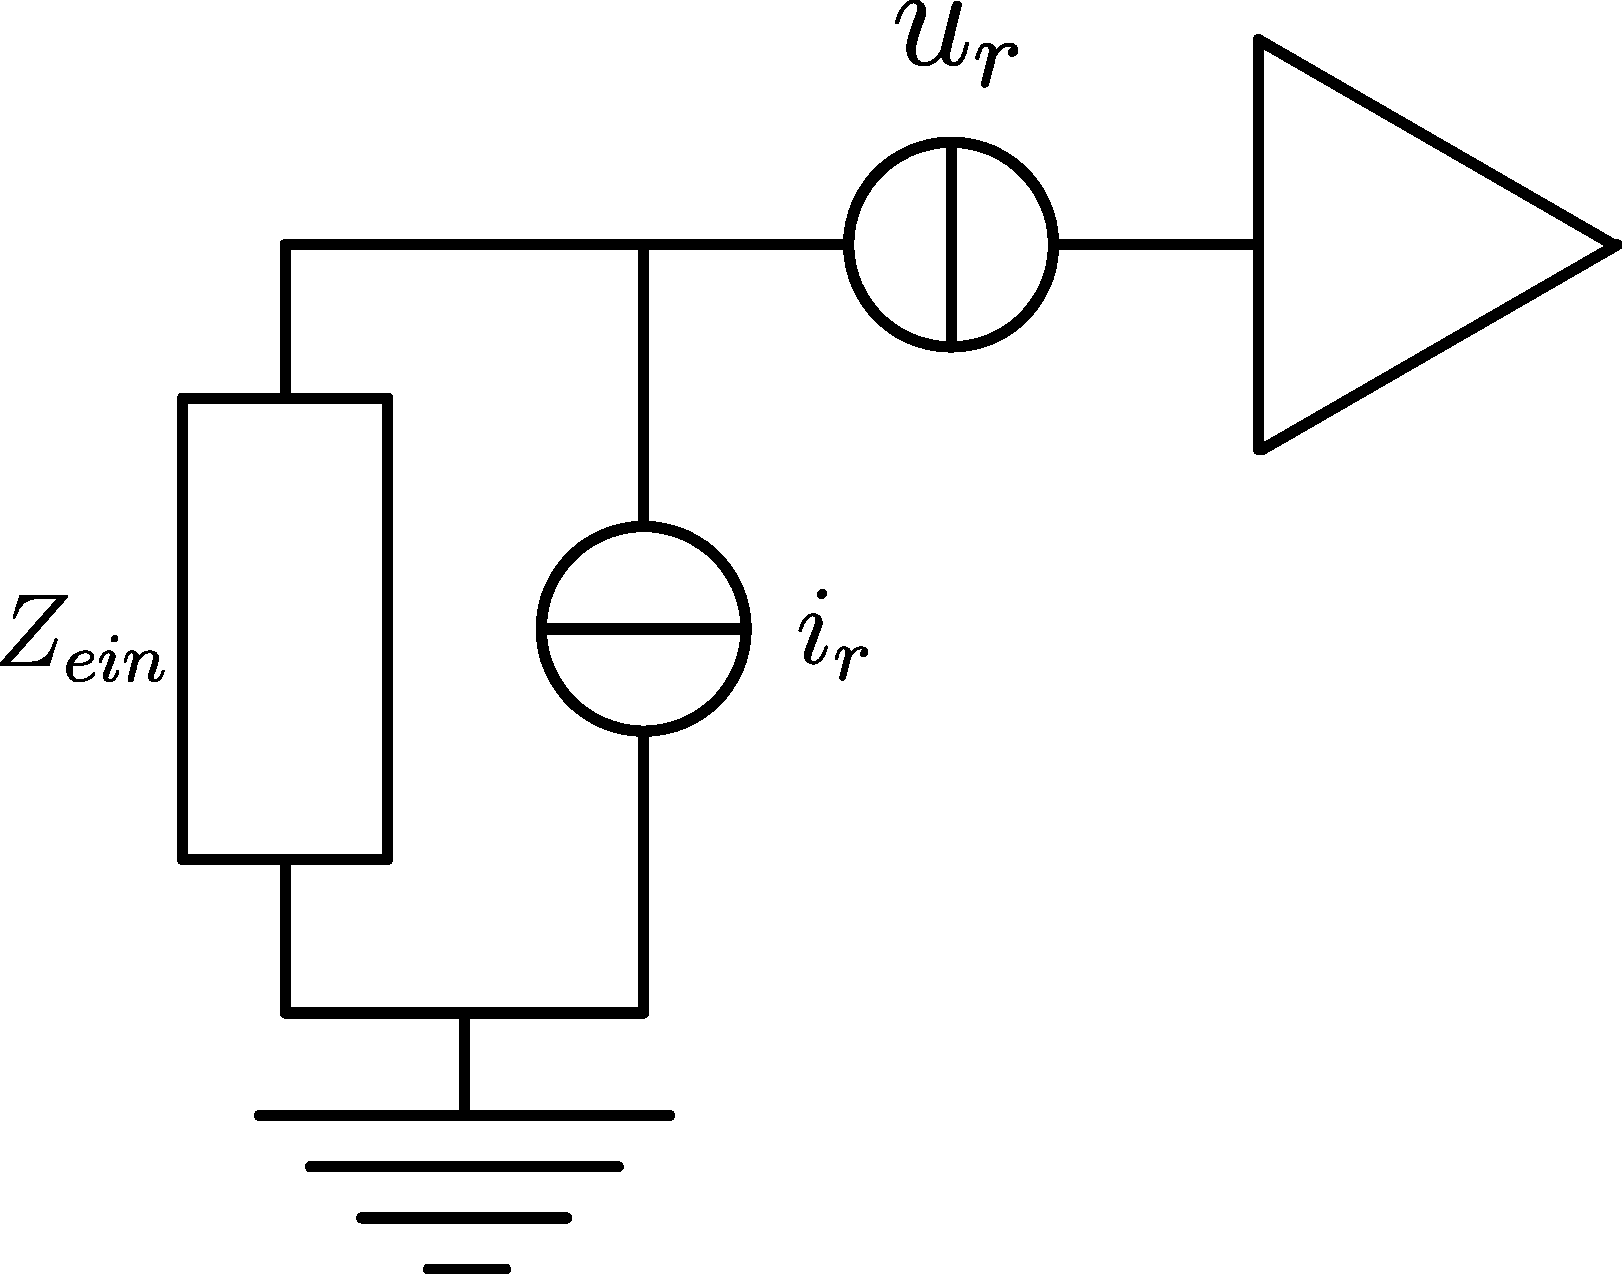
\includegraphics[width=0.50\textwidth]{./fig/NoiseSchematic.pdf}
\vspace{-0.5cm}
\caption{Ersatzschaltbild des Verstärkers.
Das Rauschen des Verstärkers wird in Form einer Rauschstromquelle $i_r$ parallel zur Eingangsimpedanz und einer Rauschspannungsquelle $u_r$ in Reihe zum Eingang eines idealen Verstärkers modelliert.
Der ideale Verstärker selbst ist frei von Rauschen.
Indem das Rauschen eingangsseitig betrachtet wird, können verschiedene Verstärker leichter verglichen werden, ohne dass die individuellen Übertragungsfunktionen berücksichtigt werden müssen.}
\label{fig:NoiseSchematic}
\end{center}
\end{figure}

\subsection*{Wärmerauschen}
Wärmerauschen entsteht in Widerständen durch die zufällige thermische Bewegung der Elektronen und ist somit im Gegensatz zum Schrotrauschen unabhängig von einem externen Strom.
Das Wärmerauschen kann im Ersatzschaltbild entweder durch eine Stromquelle parallel zum Widerstand der Größe
\begin{equation}
\stackrel{-}{i}^2 = \frac{4k_B T}{R}
\end{equation}
oder eine Spannungsquelle in Reihe zum Widerstand dargestellt werden.

\subsection*{1/f-Rauschen}
1/f-Rauschen tritt sowohl in passiven als auch in aktiven Elementen auf und liegt in vielen Ursachen begründet.
Unter anderem in der fluktuierenden Beweglichkeit der Ladungsträger.
In FETs wird 1/f-Rauschen üblicherweise als Spannungsquelle am Eingang modelliert
\begin{equation}
\stackrel{-}{e}^2 = \frac{K}{f^b}.
\end{equation}
Der Parameter $K$ ist abhängig vom Bauteil und eine Funktion des Stroms.
Der Parameter $b$ liegt in der Regel nahe bei $1$, daher der Name dieser Rauschart.

\subsection*{Verstärker Rauschen}
Das Rauschen des Verstärkers wird wie in Abb. \ref{fig:NoiseSchematic} durch die eingangsseitige Spannungsquelle $u_r$ in Reihe zum Verstärker und einer eingangsseitigen  Stromquelle $i_r$ parallel zur Eingangsimpedanz modelliert.
Die Spannungsquelle wird als ein 1/f-Rauschen und ein konstantes weißes Rauschen modelliert\cite{horowitz1980art}
\begin{equation}
u^2_r = \frac{A^2}{f} + u^2_w.
\end{equation}
Parallel zur Eingangsimpedanz ist die Rauschstromquelle $i_r$ deren Rauschen gemäß
\begin{equation}
i^2_r = a + bf + cf^2
\end{equation}
modelliert wird\cite{Thomas2016}.
Diese beschreibt den Anteil des Rauschens, welcher von der Eingangsimpedanz abhängig ist und führt zu dem Spannungsrauschen
\begin{equation}
u^2_{ri} = Z^2_{ein}i^2_r.
\end{equation}
Es wird angenommen, dass die einzelnen Rauscharten unabhängig voneinander sind und werden daher quadratisch addiert.
Das gesamte Rauschen ergibt sich somit aus dem Verstärker Rauschen, welches das thermische Rauschen beinhaltet und dem Schrotrauschen aufgrund des Leckstrom zu
\begin{align}
u_{ges} &= \frac{A^2}{f} + u^2_w + Z^2_{ein}(i^2_r + i_{Schrot}) \\
&= \left(\frac{a + 2eI_{Leck}}{4\pi^2 C^2_{ges}}\right)\frac{1}{f^2} + \left(A^2 + \frac{b}{4\pi^2 C^2_{ges}}\right)\frac{1}{f} + u^2_w + c
\label{eq:Rauschen}
\end{align}
mit $Z_{ein}$ aus Gl. \eqref{eq:EingangsC}.
